\documentclass[conference]{IEEEtran}
\IEEEoverridecommandlockouts
% The preceding line is only needed to identify funding in the first footnote. If that is unneeded, please comment it out.
\usepackage{cite}
\usepackage{amsmath,amssymb,amsfonts}
\usepackage{algorithmic}
\usepackage{graphicx}
\usepackage{textcomp}
\usepackage{xcolor}
\def\BibTeX{{\rm B\kern-.05em{\sc i\kern-.025em b}\kern-.08em
    T\kern-.1667em\lower.7ex\hbox{E}\kern-.125emX}}
\begin{document}

\title{Predicting New York City Crime Using Weather\\}

\author{\IEEEauthorblockN{Vaibhav A Gadodia}
\IEEEauthorblockA{\textit{Courant Institute of Mathematical Sciences} \\
\textit{New York University}\\
New York, New York \\
vaib@nyu.edu}
\and
\IEEEauthorblockN{Jinze Qi}
\IEEEauthorblockA{\textit{Courant Institute of Mathematical Sciences} \\
\textit{New York University}\\
New York, New York \\
jq699@nyu.edu}
}

\maketitle

\begin{abstract}
While there has been extensive work on the effect of individual weather conditions such as temperature, precipitation, etc. on the occurrence of crime and on the correlation between climate change and criminal activity, only a little research is available that attempts to forecast criminal activity using a more holistic set of weather conditions.
In this work, we aim to correlate weather combinations of temperature, relative humidity, and the presence of rain, snow, and fog with crime and predict the percentile ranks of such weather combinations and their crime risk in New York City.
\end{abstract}

\begin{IEEEkeywords}
Analytic, Application, Big Data, Crime, Spark, Weather
\end{IEEEkeywords}

\section{Introduction}
\subsection{Overview}
Crime is an unfortunate part of urban life and often millions are spent in efforts to reduce criminal activity and to safeguard citizens.
In New York City, there is a significant amount of criminal activity and the New York Police Department's attempts to protect the city residents is a big part of why the city continues to be a relatively safe place to reside despite all the crime.
However, we believe that NYPD's efforts can be enhanced by applying predictive analytics on big data and leveraging the predictive power of weather on crime.

A small body of research has shown that external factors such as temperature, precipitation, etc. influence criminal behavior significantly.
However, most of such past work has either been heavily focused on understanding the effect of individual factors on crime or has been about the correlation between weather and crime on a monthly or yearly basis.
With this work, we attempt to both explore the effect of weather as a whole on criminal behavior and study this effect on a more granular time scale of hours and minutes.

\subsection{Approach}
We explore the weather crime correlation and attempt to forecast criminal activity using weather conditions by studying local climatological and NYPD complaints data spanning a period of 12 years from the beginning of 2006 to the end of 2017.

We preprocess the data to discard irrelevant feature columns and then we combine the two cleaned datasets on the basis of date and time.
This ensures that for every complaint filed with the NYPD, we have the related weather recordings.
We then use this combined data to compute the frequency of criminal activity for different weather conditions and use that in a linear regression - with polynomial terms for modelling quadratic relationships.
We compute and report the R$^{2}$ score for each regression and use the models for crime predictions.

Our work also involves the development of an easy-to-use web application that we have built specifically for the NYPD and other NYC law enforcement agencies.
This application can be queried by the officers to obtain the expected criminal activity based on a few weather based inputs.

\subsection{Paper Organization}
This paper is organized as follows: in Section II, we describe the motivation behind this work. 
In Section III, we discuss related works.
In Section IV, we briefly describe the data used here.
In Section V, we describe our analytic, discussing preprocessing, combining data, regression analysis, and prediction.
In Section VI, we provide an overview of our application design.
In Section VII, we discuss potential actuation or remediation based on the insights gained through this analysis.
In Section VIII, we provide details on the analysis, including regression, predictions, as well as challenges and limitations of the application.

\section{Motivation}
We wanted to give the NYPD and other law enforcement agencies operating in NYC an easy to use tool for exploring the likelihood of criminal activity in the city in general and of assault, burglary and rape, in particular on any given time of day. 
Our application will assist the law enforcement officers by classifying the time of day, using weather conditions, in percentiles of expected criminal activity. 

While the application can be used by the city residents to inquire and act upon their personal safety, it has been designed with the law enforcement agencies in mind who can use the application’s output to inform their officers’ beats and take necessary action to protect citizens.

\section{Related Work}
In recent work, Alamo et. al. \cite{b1} have studied the relationship between crime in Orlando, Florida to Orlando's weather and Twitter presence.
They collected crime data as reported by the Orlando Police Department daily, which gave dates, crime categories, location, etc.
They also collected weather data from the National Oceanic and Atmospheric Administration and used a Twitter developer account to collect tweets pertaining to crime in the Orlando area.

They filtered out the tweets using specific keywords such as "crime", "larceny", etc. to isolate the tweets that have any reference to crime and used similarity measures and regression analysis to explore the relationship between crime and tweets.
Using chi-squared tests, they further concluded that high crime rates are associated with average daily temperatures over 60$^{\circ}$F and that precipitation discouraged crime.

Recently, Mullins et. al. \cite{b2} have explored the relation between ambient temperature and mental health and found that higher temperatures increase emergency department visits for mental illness and self-reported days of poor mental health.
They specifically concluded that cold temperatures reduce negative mental health outcomes while hot temperatures increase them.
Interestingly, they also conclude that there is no evidence of any adaptation and that this temperature relationship remains stable across time, base climate, air conditioning penetration rates, and other factors.

Given that mental health is a strong influence in criminal activity, these results are very significant and indicate a relation between weather and crime.

In a related work, Ranson et. al. \cite{b3} study the impact of climate change on the prevalence of criminal activity in the United States.
They use a 30-year panel of monthly crime and weather data for 2997 US counties and identify the effect of weather on monthly crime by using a semi-parametric bin estimator and controlling for state-by-month and county-by-year fixed effects.

Their results show that increasing temperature has a strong positive effect on criminal activity and they predict that between 2010 and 2099, climate change will cause more than a million additional crimes.

These works are very interesting and suggest significant external effect on criminal behavior. 
However, our work attempts to understand the effect of weather conditions as a composite instead of studying temperature, precipitation, etc. as an isolated feature and we aim to study these effects on a much more granular level of hourly observations.

\section{Datasets}
Our weather data was a part of National Center for Environmental Information's Local Climatological Data obtained at their Central Park station.
The data, which came in at about 80 MB, was downloaded once from the following link:
\underline{https://www.ncdc.noaa.gov/cdo-web/datatools/lcd}

It included entries from January 1, 2006 to December 31, 2017 and consisted of hourly recordings of dry bulb temperature, relative humidity, weather type, etc.
After cleaning the data schema was as follows:
\begin{itemize}
    \item Year: Int - The year when the weather measurement was recorded.
    \item Month: Int - The month when the weather measurement was recorded.
    \item Day: Int - The day when the weather measurement was recorded.
    \item Minute: Int - The minute when the weather measurement was recorded.
    \item Temperature: Int - The dry bulb temperature recorded.
    \item Rain: Int - 0/1 entry indicating absence/presence of rain.
    \item Snow: Int - 0/1 entry indicating absence/presence of snow.
    \item Fog: Int - 0/1 entry indicating absence/presence of fog.
    \item Humidity: Int - The relative humidity recorded.
\end{itemize}

The second data that we used was the historical complaint data made available by the NYPD.
This data, which came in at about 2 GB was collected once from the following link:
\underline{https://data.cityofnewyork.us/Public-Safety/NYPD- Complaint}
\underline{-Data-Historic/qgea-i56i}

It had entries from January 1, 2006 to December 31, 2017 and tracked all complaints filed with the NYPD over this 12 year period and consisted of crime location, latitude, longitude, crime type, etc.
After cleaning the data schema here was as follows:
\begin{itemize}
    \item Year: Int - The year of the occurrence of the reported crime.
    \item Month: Int - The month of the occurrence of the reported crime.
    \item Day: Int - The day of the occurrence of the reported crime.
    \item Minute: Int - The minute of the occurrence of the reported crime.
    \item Crime Type: Int - The type of crime reported. Each unique type was indicated by a numeric code, for instance, assault was 9, burglary had 3 as its numeric code, rape was number 45, etc.
\end{itemize}

\section{Description of Analytic}
\begin{figure*}[htbp]
\centerline{\scalebox{0.5}{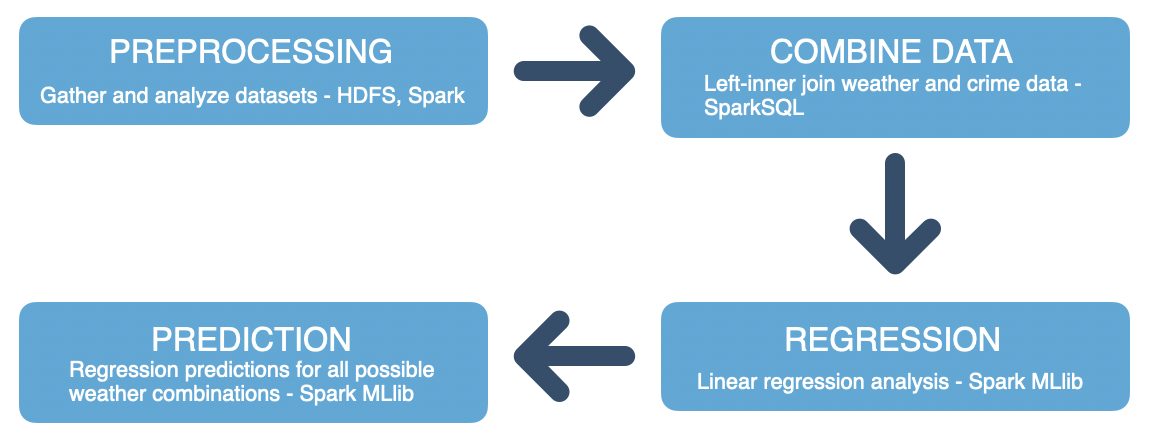
\includegraphics{design_diagram.png}}}
\caption{Analytic Design}
\label{design}
\end{figure*}

\subsection{Preprocessing}
We preprocessed the weather data using an Apache Spark pipeline. 
We filtered out all feature columns that were either deemed to be non-essential based on domain knowledge or those that did not have any recorded readings for multiple years in the period spanned by our data. 
As a consequence of this filtering, our data was left with four feature columns that were further processed and are described below.
\begin{itemize}
    \item DATE: The values here indicated the date and time when the weather measurements were recorded. The values included the data - in YYYY-MM-DD format - concatenated with time - in HH:MM format - with a "T". 
    We further processed this column and split it into four different features indicating year, month, day and time (in minutes based on a 24-hour clock starting at 0 minutes at 00:00 hours). 
    We rounded off the minutes to the nearest 60.
    \item HourlyDryBulbTemperature: This feature column had the dry bulb temperature readings recorded by the automated sensors. 
    The values were in whole degrees Fahrenheit and ranged from low negatives to over a $100^{\circ}$F.
    \item HourlyPresentWeatherType: The values here indicated observed weather types using AU, AW and MW codes. 
    For instance, "RA" indicated rain, "FG" indicated fog, etc. We processed this column and split it into three separate categorical columns for rain, snow and fog, with binary 0/1 values indicating the absence/presence of the relevant weather type.
    \item HourlyRelativeHumidity: This was the observed relative humidity given to the closest whole percentage.
\end{itemize}

After filtering out irrelevant feature columns, the weather data was further processed and the observations with irregular data entries were discarded.
This included entries where either the temperature or relative humidity readings were left out or those that had irrelevant wildcard characters in their recordings such as "*", "s", etc.

For the crime data, we used a similar Apache Spark pipeline for preprocessing.
We began by filtering out non-essential feature columns, which left us with three that were further processed and are described below.
\begin{itemize}
    \item CMPLNT\_FR\_DT: The values here indicated the date of the occurrence of the reported crime.
    The values were in MM/DD/YYYY format and we split these into three separate columns for year, month and day.
    \item CMPLNT\_FR\_TM: This column had the time of the occurrence of the reportec crime in HH:MM:SS format, which we converted into minutes like in the weather data.
    \item OFNS\_DESC: The values here indicated the type of crime reported.
    These were names of different crime types, which we converted into integers by assigning each one of the 71 types a numerical code from 0 to 70.
\end{itemize}

After the aforementioned processing, we removed all rows with irregular or missing entries.

\subsection{Combining Data}
In order to relate the crime data with the weather conditions when the complaint was filed, we generated two SparkSQL DataFrames for the preprocessed weather and crime datasets. 
These were then combined using a "left-inner" join according to the two dataframes' year, month, day and minutes columns. 
This generated a combined dataset for analysis and ensured that every crime reported was associated with the relevant weather conditions.

\subsection{Regression}
We used the newly combined dataset to compute the total complaints filed for each weather condition - which was a combination of the temperature, relative humidity, rain, snow and fog - and the complaints filed for each weather condition that were specifically related to assault, burglary and rape.
This way we ended up with four input datasets that were used in a linear regression for analysis of the impact of weather conditions on criminal activity and to predict future crime rate.

For our regression analysis, we used Apache Spark's MLlib's LinearRegression model.
For all four regression models, the weather conditions were treated as the independent variables and included temperature and relative humidity as continuous variables and rain, snow and fog as categorical dummy variables. 
Additionally, two polynomial terms comprising of the squared temperature  and squared relative humidity were also included as independent variables.
These additional polynomial terms ensured the regressions' ability to model non-linear quadratic relationship between weather and crime that was observed in preliminary exploration and visualization of the data.
For our models, the dependent variables were one of the number of overall crimes, number of assaults, number of burglaries, or the number of rapes.
Therefore, the models took the following form.
\begin{multline}\label{eq}
    \#crimes = \theta_{0}temp + \theta_{1}temp^{2} + \theta_{2}rain + \theta_{3}snow + \\
    \theta_{4}fog + \theta_{5}humidity + \theta_{6}humidity^{2}
\end{multline}

\subsection{Prediction}
Given these four regression models, we are able to predict the number of expected crimes for every possible weather condition and then convert those values into percentiles to determine criminal risk.

\section{Application Design}
\begin{figure*}[htbp]
\centerline{\scalebox{0.25}{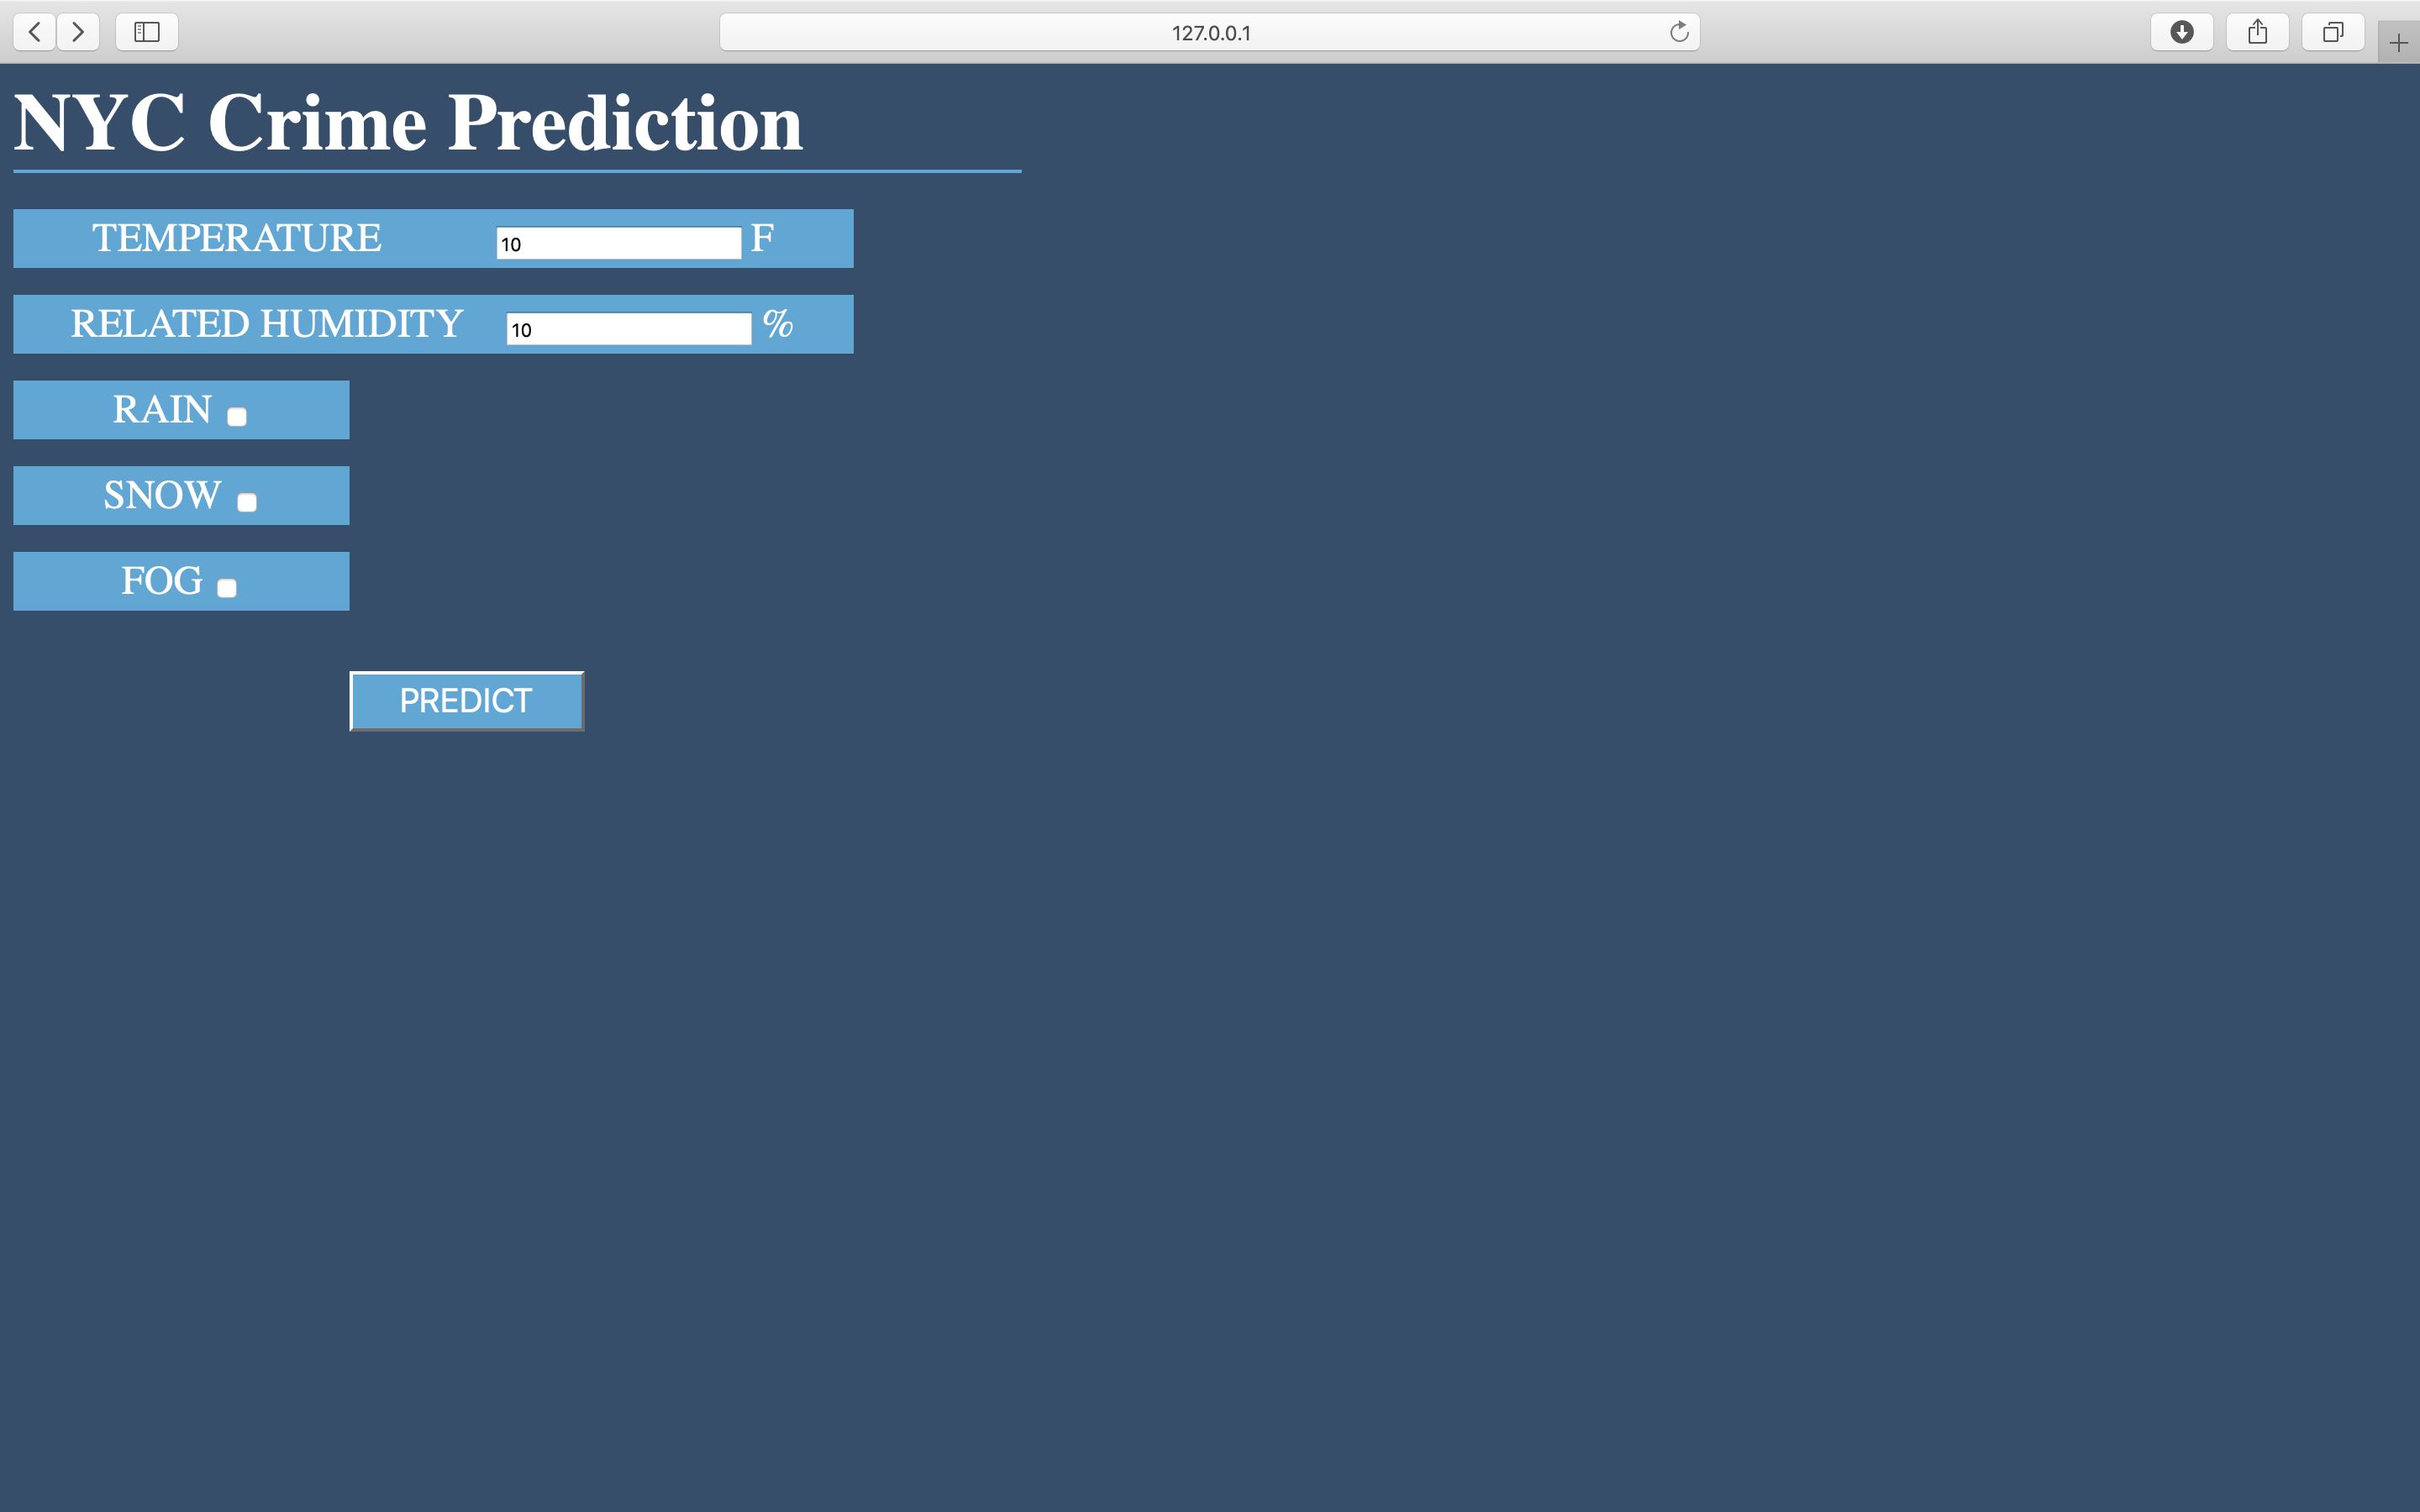
\includegraphics{app_in.png}}}
\caption{Application - Input}
\label{design}
\end{figure*}

\begin{figure*}[htbp]
\centerline{\scalebox{0.25}{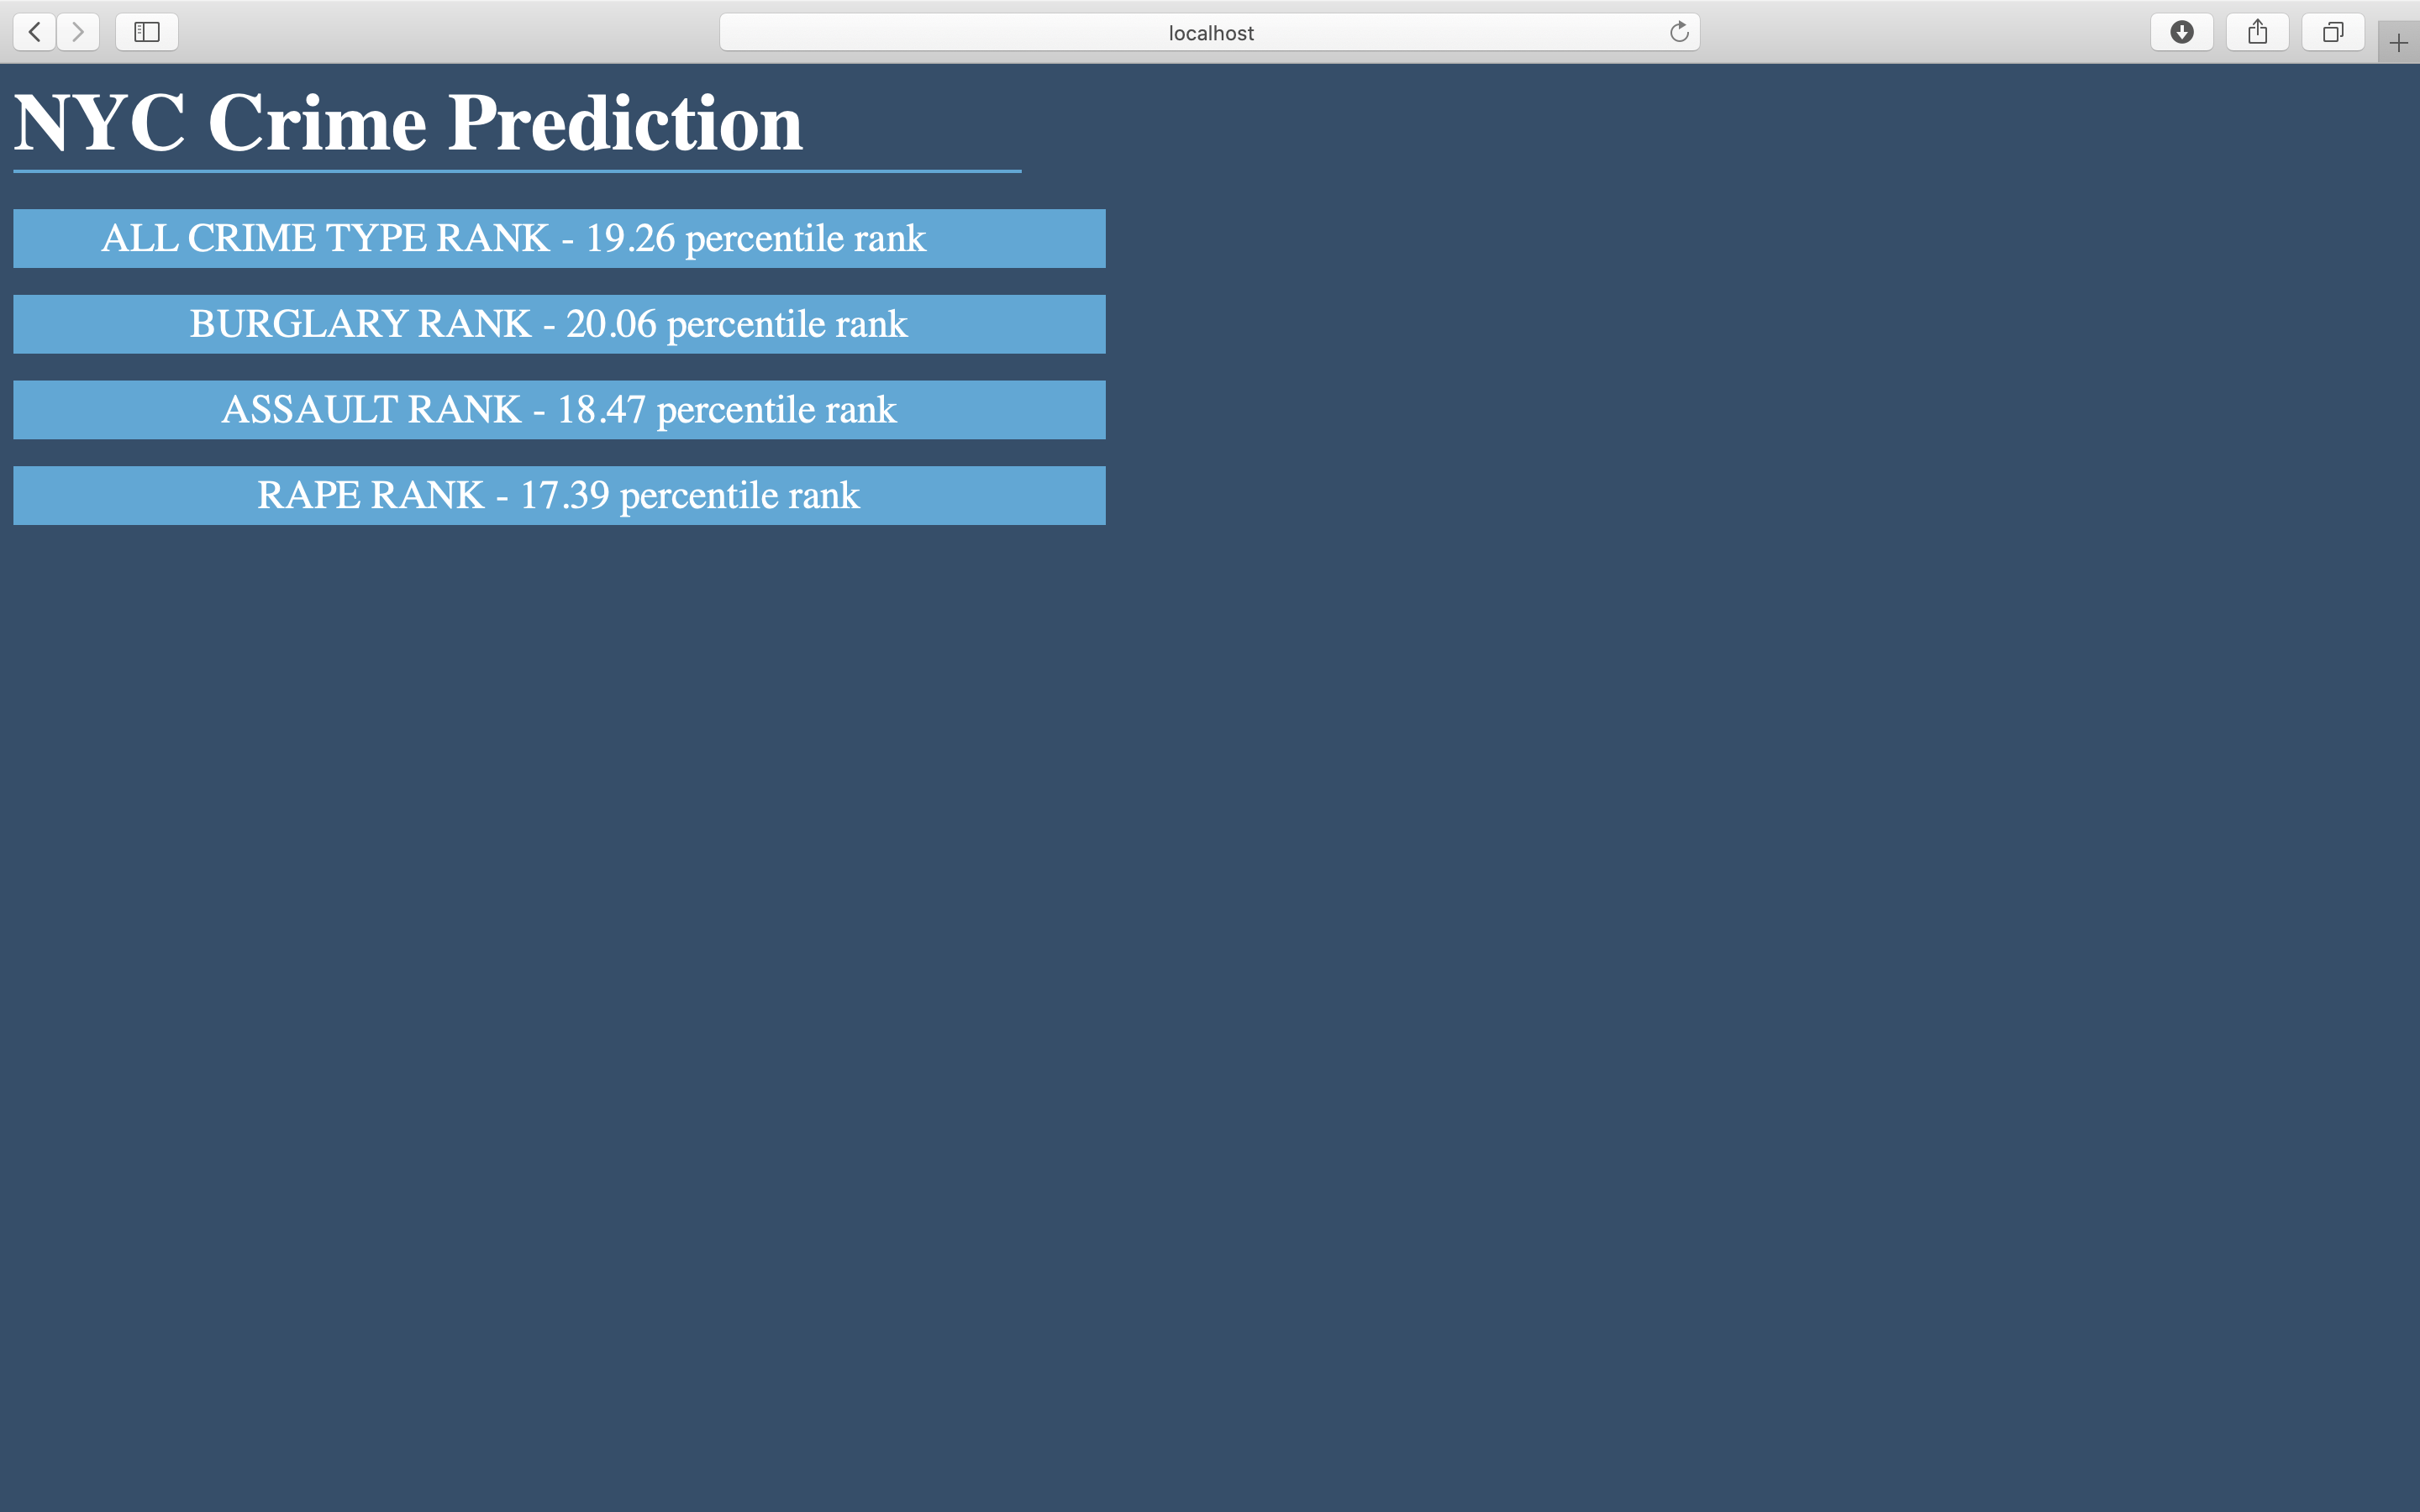
\includegraphics{app_out.png}}}
\caption{Application - Output}
\label{design}
\end{figure*}

The workflow for the backend of this project has been illustrated in Fig. 1.
We began the work by gathering, analyzing and cleaning the data, which was followed by the generation of a combined dataset and performing regression analysis on it.
Finally, we used the regression models to predict crime rates.

The primary goal of this project was to enable the NYPD in keeping the city safer.
As a consequence, we wanted to provide them with an easy-to-use application powered by a strong analytic.
Thus, in addition to the backend, we also created a simple Flask based web application.
The NYPD can query this application to forecast criminal risk by entering the observed weather conditions as shown in Fig. 2 and the application provided them with a straightforward forecast as shown in Fig. 3.

\section{Actuation or Remediation}
When a law enforcement official queries our application inputting the observed weather conditions, our application returns a percentile ranking of the conditions' criminal risk.
The officers can use this ranking to inform their department's beats and to increase/decrease police presence in high risk neighborhoods.
Furthermore, on a longer time scale, this application's insights can be used by the law enforcement agencies to inform their budgeting and recruiting efforts.

\section{Analysis}

\begin{table*}[htbp]
\caption{Regression R$^{2}$ Scores}
\begin{center}
\begin{tabular}{|c|c|c|c|c|}
\hline
& \textbf{Overall} & \textbf{Assault} & \textbf{Burglary} & \textbf{Rape} \\
\hline
\textbf{R$^{2}$} & 0.4037 & 0.4185 & 0.3717 & 0.2796 \\
\hline
\end{tabular}
\label{r2}
\end{center}
\end{table*}

\subsection{Regression}
Given the combined weather and crime dataframe, we computed the total number of crimes for each observed weather combination of temperature, relative humidity, rain, snow, and fog that was available in the data.
We repeated this step for the other three regression models as well where we calculated the total number of assaults, burglaries, and rapes for each observed weather combination present in the data.
After including the additional polynomial terms in our regression models, we performed linear regression analysis on all four dataframes.

The trained models had coefficients of determination - R$^{2}$ scores - that are shown in TABLE~\ref{r2}. 
While the R$^{2}$ scores might appear to be low, one must take into account the affect of non-weather related factors on human activity, in general and on crime, in particular.
These scores suggest a reasonable correlation between weather conditions as a whole and criminal activity.
Furthermore, our analysis suggests that among assault, burglary, and rape, assault has the highest correlation with weather and it is even higher than the overall crime rate's correlation with weather conditions.
On the other hand, both burglary and rape have a lower correlation with weather, with rape being the least strongly affected by it.

\subsection{Prediction}
We used our trained models to predict criminal activity for all possible weather combinations.
In order to do so in a reasonable manner, we rounded off the temperature and relative humidity values to the nearest ten, thus limiting the total possible weather combinations to 880.
This does not significantly alter the model predictions as there is no significant change within a few degrees of temperature or percentages of relative humidity.

\subsection{Challenges and Limitations}
Our regression models provide a reliable framework for forecasting crimes using weather conditions.
However, due to the nature of regression analysis, there were challenges in how the predictions were to be interpreted and presented to the user.
\begin{itemize}
    \item Due to the nature of regression analysis, some predictions tend to be negative.
    However, this is not an indicator of a complete lack of criminal activity.
    Rather, this is an artifact of regression based predictions and therefore, was treated as such because we converted the predictions into percentiles.
    \item Another closely related limitation of the application was that the regression prediction shows the expected number of crimes over a 12 year period.
    This is an artifact of the data used for analysis as it spanned 12 years from January 1, 2006 to December 31, 2017.
\end{itemize}
For the aforementioned reasons, our application does not present the user with the raw regression prediction.
Instead, we present the user with a percentile rating of the input weather conditions' criminal risk based on the regression predictions of all possible weather conditions.
This comes with its own set of challenges as not all combinations of temperature, humidity, rain, snow, and fog are physically possible.
However, this is a reasonable approximation that helps prevent misinterpretation of the application output.

The crime data used for regression analysis was organized by the date and time of the crime that was reported in the complaints filed with the NYPD.
This presents significant challenges as there is no way of informing our analysis whether the time of crime as reported in the complaints were accurate or not.
This affects our models as this raises the possibility of there being entries in our data where the correct weather conditions are not matched to the crime and therefore, this ultimately affects our predictions.

\section{Conclusion}
Crime is an unfortunate reality of urban life and NYC has seen more than its fair share of criminal activity over the years.
A lot of work has been done by the law enforcement agencies and city government to protect vulnerable citizens.
Our results show that these efforts could be further enhanced by using the predictive power of weather conditions on NYC crime.

We found that temperature, relative humidity, rain, snow, and fog have a significant influence on crime.
Our regression models further isolated assault, burglary, and rape and we found that the aforementioned weather conditions significantly affected these crimes, albeit to varying degrees.

In addition to data analysis, we also developed an easy-to-use web application that can be employed by the law enforcement arm of the government to inform their work.

\section{Future Work}
\textit{1) Taking correctness of complaints into account:} While our models are reasonably functional in their current form , they do not take into account the possibility of there being false or incorrect complaints that could cause discrepancies in important information such as the date and time of actual crimes and when the complaints indicated they happened.
Since, our analysis is informed by the weather conditions at the moment of crimes, there is a possibility that our predictions could be further improved if such discrepancies were taken into account.

\textit{2) More complex modelling techniques:} Given the structure of our data, linear regression with polynomial terms was the best way of modelling relationship between weather and crime.
However, it would be interesting to further explore this relationship using advanced modern techniques such as Deep Learning, random forest analysis, etc.

\textit{3) Predicting type of crime with highest probability:} We currently predict the number of crimes that are expected for a given weather combination over a span of 12 years.
However, it would be very interesting and useful to develop a model to predict the types of crimes with the highest probabilities of occurring in particular weather conditions.

\begin{thebibliography}{00}
\bibitem{b1}J. Alamo, C. Fortes, N. Occhiogrosso, and C.-Y. Huang, “Mining the Relationship between Crimes, Weather and Tweets,” Proceedings of the 2019 the International Conference on Pattern Recognition and Artificial Intelligence - PRAI 19, 2019.
\bibitem{b2}J. T. Mullins and C. White, “Temperature and mental health: Evidence from the spectrum of mental health outcomes,” Journal of Health Economics, vol. 68, Dec. 2019.
\bibitem{b3}M. Ranson, “Crime, weather, and climate change,” Journal of Environmental Economics and Management, vol. 67, no. 3, pp. 2734–302, May 2014.
\end{thebibliography}
\end{document}
